\section{Auswertung}
\label{sec:Auswertung}

Im folgenden wird zunächst die Winkelrichtgröße $D$ und das Eigentraegheitsmoment der drehachse bestimmt.
Dazu Messen wir die rücktreibende kraft $\symbf{F}$ der Spiralfeder für verschiedene auslenkungen $\Phi$.


\begin{table}
  \centering
  \caption{Messwerte zur bestimmung von $D$.}
  \label{tab:tabelle}
  %\sisetup{table-format=1.1, per-mode=reciprocal}
  \begin{tblr}{
      colspec = {S S },
      row{1} = {guard, mode=math},
      %vline{4} = {2}{-}{text=\clap{$\pm$}},
    }
    \toprule
    \Phi &  F(N)\\
    \midrule
    22.5  & 0\\
    45    &0.04\\
    67.5  &0.068\\
    90    & 0.09\\
    112.5 &0.126\\
    135   &0.164\\
    157.5 & 0.172\\
    180   & 0.18\\
    202.5 & 0.2\\
    225   & 0.28\\
    \midrule
    $\overline{\Phi}$& $\overline{F(N)}$\\
    \midrule
    \bottomrule
  \end{tblr}
\end{table}

mit diesen mittelwert kann man mit Formel \autoref{} und $r= ???cm$ Die Winkelrichtgröße 
der Spiralfeder zu ???? bestimmen. 

Als nächstes wird das Eigenträgheitsmoment $I_D$ der Drillachse bestimmt. Dazu wird Das Trägheitsmoment 
eines Dünnen stabes mit 2 identischen liegenden Hohlzylindern im abstand a von der Drehachse 
zusammen mit dem Trägheitsmoment der Drillachse bestimmt, um danach den Theoretischen wert von dem dünnen Stab mit den zwei Hohlzylindern 
abziehen zu können und das Trägheitsmoment von der Drillachse zu erhlten.



\begin{table}
  \centering
  \caption{Messwerte T/a.}
  \label{tab:tabelle}
  %\sisetup{table-format=1.1, per-mode=reciprocal}
  \begin{tblr}{
      colspec = {S S },
      row{1} = {guard, mode=math},
      %vline{4} = {2}{-}{text=\clap{$\pm$}},
    }
    \toprule
    \Phi &  F(N)\\
    \midrule
    5&4\\
    \midrule
    $\overline{\Phi}$& $\overline{F(N)}$\\
    \midrule
    \bottomrule
  \end{tblr}
\end{table}










\begin{figure}
  \centering
  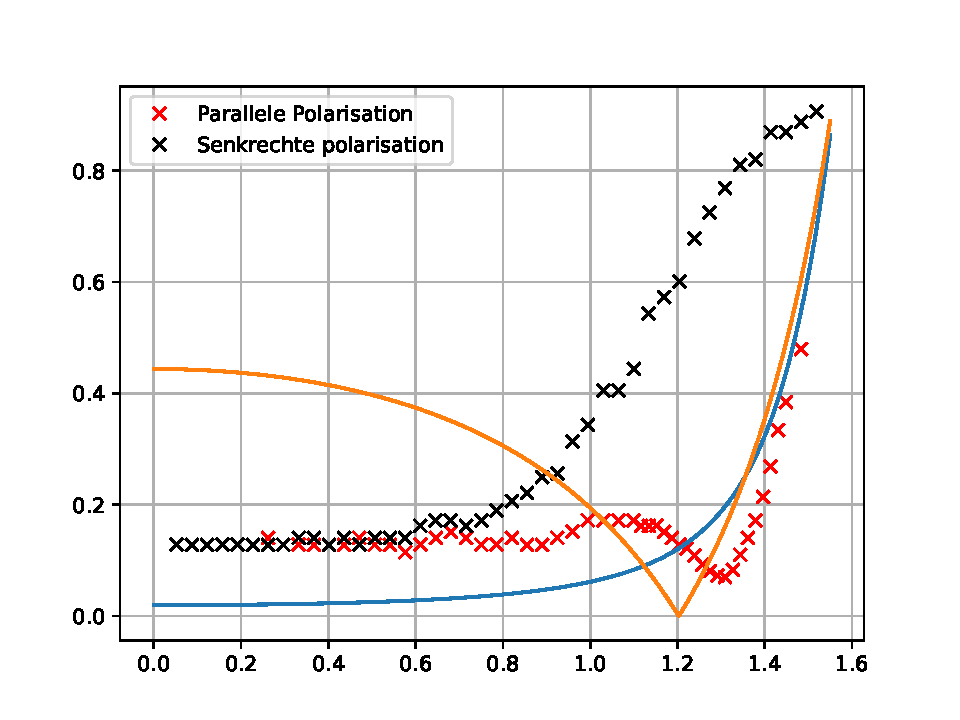
\includegraphics{plot.pdf}
  \caption{Plot.}
  \label{fig:plot}
\end{figure}


